\documentclass[a4paper]{article}
\usepackage[utf8x]{inputenc}
\usepackage[russian]{babel}
\usepackage{multicol}
\usepackage[warn]{mathtext}
\usepackage{graphicx}
\usepackage{wrapfig}

\usepackage{lipsum}
\usepackage{amsmath}
\usepackage{floatflt}
\usepackage{geometry} \geometry{verbose,a4paper,tmargin=2cm,bmargin=2cm,lmargin=2.5cm,rmargin=1.5cm}
\usepackage{float}
\usepackage{amssymb}
\graphicspath{{}}
\usepackage{caption}

\begin{document}

\begin{titlepage}
	\centering
	\vspace{5cm}
	{\scshape\LARGE Московский физико-технический институт \par}
	\vspace{4cm}
	{\scshape\Large Вопрос по выбору \par}
	\vspace{1cm}
	{\huge\bfseries  Фазовые переходы в сегнетоэлектриках и устройство FeRAM \par}
	\vspace{1cm}
	\vfill
\begin{flushright}
	{\large выполнил студент 852 группы ФФКЭ}\par
	\vspace{0.3cm}
	{\LARGE Водзяновский Яромир}
\end{flushright}
	
	\vfill

% Bottom of the page
	Долгопрудный, 2020 г.
\end{titlepage}

\newpage

\tableofcontents

\newpage

\section{Введение} 

\subsection{Основные понятия}

\textbf{Сегнетоэлектрики} -  вещества, обладающие спонтанной поляризацией, направление которой может быть изменено с помощью внешнего электрического поля. 

Сегнетоэлектрики обладают рядом специфических свойств, которые проявляются лишь в определенном диапазоне температур:

\begin{itemize}

\item

\textbf{$T < T_c$}

Температура $T_c$ (сегнетоэлектрическая точка Кюри) является температурой фазового перехода, ниже этой температуры сегнетоэлектрик обладает доменной структурой и характерными сегнетоэлектрическими свойствами:

\begin{itemize}

\item

Нелинейная зависимость их поляризованности или электрической индукции от напряженности электрического поля $\vec{E}$, которая носит название диэлектрической петли гистерезиса (Рис. \ref{p1})

\begin{equation}
\chi = \frac{\partial P}{\partial E},
\label{1}
\end{equation}

\begin{equation}
\varepsilon = 1 + 4\pi \chi,
\label{2}
\end{equation}

где $\chi$ - поляризуемость, $\varepsilon$ - диэлектрическая проницаемость. 
Стоит отметить, что из-за анизотропии кристалла поляризуемость $\chi$ есть тензор, но для простоты мы будем этим пренебрегать. 

\item

Резко выраженная температурная зависимость диэлектрической проницаемости, в которой максимум диэлектрической проницаемости достигается при температуре, соответствующей точке Кюри.

Значение диэлектрической проницаемости в полярной фазе аномально велики. Для сегнетовой соли в максимуме $\varepsilon \approx 10000$, для титаната бария $\varepsilon \approx 6000 - 7000$. 

\item

В полярной фазе центр положительных зарядов всего кристалла не совпадает с центром отрицательных, т.е. имеется макроскопический дипольный момент. 

\end{itemize}

\item

$T > T_c$

Выше температуры Кюри происходит распад доменной структуры и сегнетоэлектрик переходит в параэлектрическое состояние. 

В неполярной фазе сегнетоэлектрик ведет себя как обычный линейный диэлектрик, в котором поляризация пропорциональна полю. Однако поляризуемость $\alpha$ и диэлектрическая проницаемость $\varepsilon$ меняются с температурой. Вблизи точки Кюри имеет место закон Кюри-Вейса:

$$\alpha = \frac{C}{T - T_0}$$

где $C$ и $T_0$ - постоянная Кюри и температура Кюри-Вейса соответственно. $T_0$ мало отличается от температуры Кюри $T_c$, при которой происходит фазовый переход из полярной фазы в неполярную. 

\end{itemize}

\begin{wrapfigure}[12]{r}{150pt}
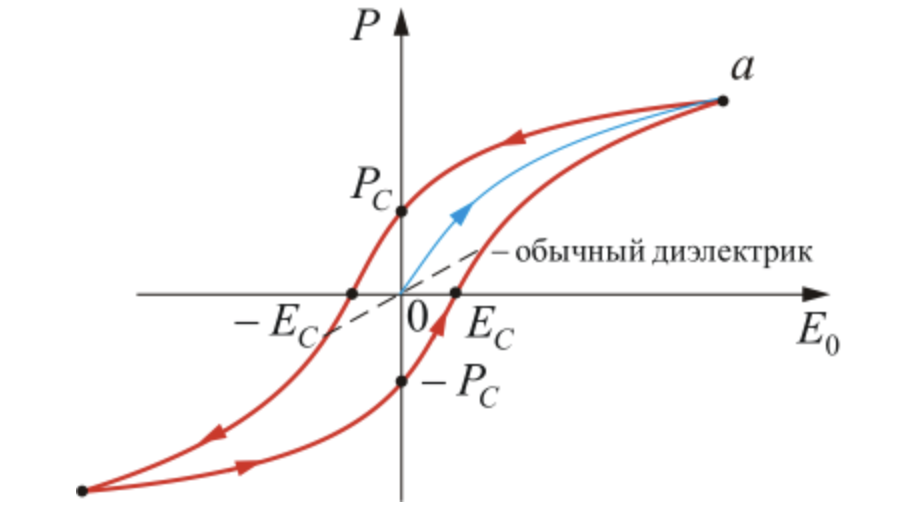
\includegraphics[scale = 0.4]{p1.png}
\caption{Сегнетоэлектрический гистерезис}
\label{p1}
\end{wrapfigure}

Как правило, сегнетоэлектрик имеет только одну точку Кюри, ниже которой он находится в полярной, а выше - в неполярной фазе. Исключение составляют сегнетова соль и изоморфные с ней соединения, а также соли $Ag_2H_3IO_6$ и $Ag_2D_3IO_6$. Они имеют две точки Кюри, между которыми и наблюдается спонтанная поляризация. 


\subsection{Доменная структура}

Существование доменов объясняется дефектами и стремлением кристалла к минимуму внутренней энергии. При возникновении спонтанной поляризации на внешней поверхности кристалла появляются поверхностные заряды ,которые, в свою очередь, должны создать внешнее деполяризующее поле, которое будет стремится однородную поляризацию; в результате, кристалл разбивается на домены, т.е. области, в которых векторы поляризации антипараллельны. Это состояние энергетически выгоднее, т.к. уменьшается деполяризующее поле. Стабильная поляризация доменов установится при достижении энергетического баланса между процессами образования доменных стенок и деполяризующего поля. 

Существуют несколько типов доменных структур:

\begin{itemize}

\item

Если сегнетоэлектрик имеет одну полярную ось, то возможны только два взаимно противоположных направления поляризации доменов параллельные этой оси. (рис. \ref{p4} а)

На этом примере хорошо видно, что электрическое поле, созданное спонтанной поляризацией одной части образца, воздействует на поляризацию другой части так, что энергетически выгоднее противоположная поляризация этих двух частей. 

\item

В одном домене дипольные моменты направлены одинаково, но в соседних доменах направлены различно. (рис. \ref{p4} б)

\item

В сегнетоэлектриках с несколькими полярными осями доменная структура более разнообразна. 

\end{itemize}


\begin{figure}[H]
\begin{center}
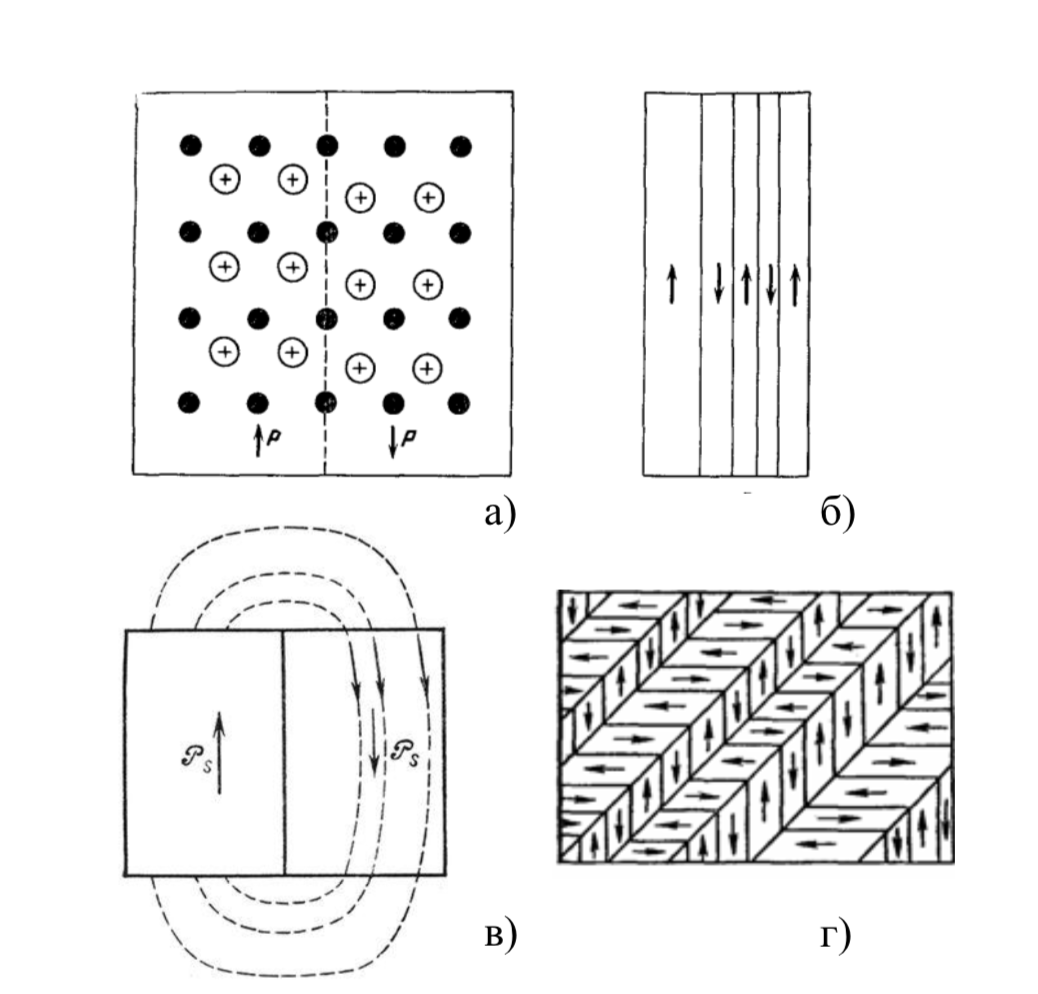
\includegraphics[scale = 0.35]{p4.png}

\caption{а) Схема смещений по обе стороны доменной границы, разделяющей домены противоположной поляризации; б) структура с доменами противоположной поляризации; в) Взаимодействие электричество поля $\vec{E}$ с одной части образца со спонтанной поляризацией другой его части; г) возможная доменная структура в двухосном сегнетоэлектрике}
\label{p4}
\end{center}
\end{figure}

Суммарная поляризация определяется разностью объемов доменов с противоположными направлениями поляризации. 


\section{Фазовые переходы в сегнетоэлектриках}

В основе теории Ландау лежит представление о фазовом переходе, который происходит в результате изменения симметрии, а не агрегатного состояния тела. Симметрия системы описывается фактором упорядоченности $\eta (p, T)$ (p соответствует давлению), который равен нулю в неупорядоченной фазе и отличен от нуля, характеризующихся более низкой фазой. 

\

\textbf{Фазовые переходы} первого и второго рода:

\begin{itemize}

\item
Если при изменении температуры фактор упорядоченности $\eta$ изменяется скачком, то имеет место фазовый переход 1-го рода (\textbf{ФП-1})

\item
Если фактор $\eta$ меняется непрерывно, то имеет место фазовый переход 2-го рода (\textbf{ФП-2})
\end{itemize}

\

В феноменологической теории сегнетоэлектриков чаще пользуются полным термодинамическим потенциалом:

\begin{equation}
F = U - TS + pV - PE,
\label{3}
\end{equation}

\begin{equation}
dF = -SdT + Vdp - P_iE_i,
\label{4}
\end{equation}

$P_i, E_i$ - компоненты векторов P и E (i = 1,2,3)

\

Из ур-й (\ref{1}, \ref{4}) c точки зрения изменения электрических величин, к сегнетоэлектрикам с ФП-1 относятсе те, которые испытывают скачки поляризации 

\begin{equation}
P_i =- \left( \frac{\partial F}{\partial E} \right)_{p, T},
\label{7}
\end{equation}

а к сегнетоэлектрикам с ФП-2, т.е., у которых скачком изменяется диэлектрическая восприимчивость

\begin{equation}
\chi_i =- \left( \frac{\partial^2 F}{\partial^2 E_i} \right)_{p, T}
\label{8}
\end{equation}

\ 

\newcommand{\RNumb}[1]{\uppercase\expandafter{\romannumeral #1\relax}}

\subsection{Фазовый переход \RNumb{2} рода}

Рассмотрим теорию фазовых переходов \RNumb{2} рода Ландау, в применении к сегнетоэлектрикам её развили В.Л. Гинcбург и А.Ф. Девоншир. 

 \
 
Гинсбург ввел величину квадрата спонтанной поляризации $P^2_s$. Важнейшее допущение состоит в том, что термодинамический потенциал F можно разложить по степеням параметра порядка. 
 
 
 
Для одномерного случая симметричного кристалла возможны только две ориентации спонтанной поляризации $\pm P_s$. Поскольку оба направления равноправны, то в разложении свободной энергии будут присутствовать члены только с четными степенями:

\begin{equation}
F = F_0 + \frac{\alpha}{2} P^2 + \frac{\beta}{4} P^4 + \frac{\gamma}{6} P^6 + \ldots
\label{9}
\end{equation}

где $F_0$ - свободная энергия в параэлектрической фазе, P - поляризация, $\alpha , \beta , \gamma$ - коэффициенты разложения, зависящие от температуры и давления. 

\

Так как равновесные условия соответствуют минимуму свободной энергии F, тогда из (\ref{4}) $E = \frac{\partial F}{\partial P}$ и условие минимума $\frac{\partial F}{\partial P} = 0$; $\frac{\partial^2 F}{\partial P^2} > 0$, то находим:

\begin{equation}
E = \alpha P + \beta P^3 + \gamma P^5,
\label{10}
\end{equation}

\begin{equation}
\alpha + 3\beta P^2 + 5\gamma P^4 > 0.
\label{11}
\end{equation}

Если внешнее поле E = 0, то пропадет индуцированная поляризация и  (\ref{10}) и (\ref{11}) примут вид:

\begin{equation}
\alpha P_s + \beta P^3_s + \gamma P^5_s = 0,
\label{12}
\end{equation}

\begin{equation}
\alpha + 3\beta P^2_s + 5\gamma P^4_s > 0. 
\label{13}
\end{equation}

При $T > T_c$ фаза находится в устойчивом параэлектрическом состоянии, и из решения ур-й (\ref{12}) и (\ref{13}) следует, что при 

\begin{equation}
P_s = 0 \; \; \; \alpha > 0. 
\label{14}
\end{equation}

Ниже точки Кюри, когда $T < T_c$ и существует сегнетоэлектрическая фаза, $P_s \neq 0$. Тогда из тех же уравнений следует, что при сохранении членов только до 4-го порядка:

\begin{equation}
P^2_s = -\frac{\alpha}{3 \beta} \; \; \text{и} \; \; \alpha < 0. 
\label{15}
\end{equation}

Отметим, что коэффициент $\beta > 0$ из условий минимума F.  

Если $\alpha$ изменяется непрерывно от $\alpha > 0$ до $\alpha < 0$ при переходе из параэлектрической фазы в сегнетоэлектрическую, то при $T = T_c$   $\alpha_{T_c} = 0$. Вблизи перехода можно принять:

\begin{equation}
\alpha = \frac{\partial \alpha}{\partial T} (T - T_c) = \alpha'_{T_c} (T - T_c)
\label{16}
\end{equation}

Отсюда

\begin{equation}
P^2_s = \frac{\alpha'_{T_c}}{3\beta} (T - T_c). 
\label{17}
\end{equation}

$\alpha$ и $\beta$ являются параметрами спонтанной поляризации. 

\ 

Зависимость для сегнетоэлектрического перехода \RNumb{2} рода приведена на Рис. \ref{p5} 

\begin{figure}[H]
\begin{center}
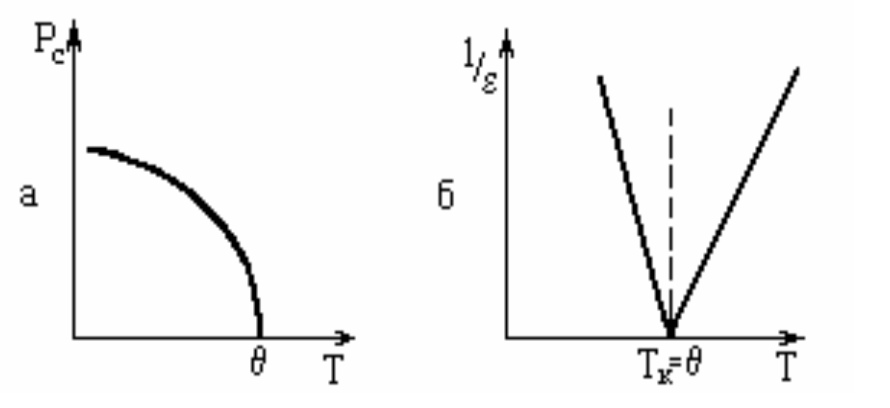
\includegraphics[scale = 0.7]{p5.png}

\caption{Температурные зависимости спонтанной поляризации (а) и обратной диэлектрической проницаемости (б) в сегнетоэлектриках с ФП-2}
\label{p5}
\end{center}
\end{figure} 

\begin{figure}[H]
\begin{center}
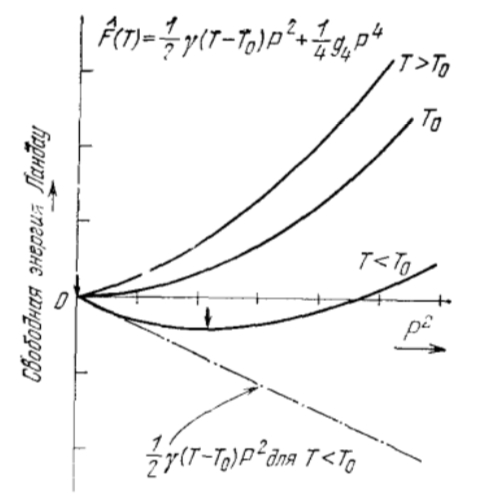
\includegraphics[scale = 0.7]{p6.png}
\caption{Свободная энергия Ландау как функция квадрата поляризации при различных температурах. Когда температура падает ниже $T_0 = T_c$ равновесное значение поляризации постепенно возрастает, что естественно отвечает минимуму свободной энергии.}
\label{p6}
\end{center}
\end{figure}


При $T > T_c$ в области параэлектрической фазы и слабых полях, выполняется зависимость $E = \alpha P$ (из ур-я (\ref{10})). В разложении можем пренебречь членом $P^3_c$. Тогда диэлектрическая восприимчивость:

\begin{equation}
\chi_+  = \frac{\partial P}{\partial E} = \frac{1}{\alpha} = \frac{1}{\alpha'_{T_c} (T - T_c)} = \frac{C}{(T - T_c)}. 
\label{18}
\end{equation}

Уравнение (\ref{18}) для $T > T_c$ представляет собой закон Кюри-Вейсса, а коэффициент $\alpha $ равен обратной диэлектрической проницаемости. 

 \
 
При $T < T_c$:
 
 \begin{equation}
E = \alpha P + \beta P^3. 
\label{19}
\end{equation}

Учитывая, что $P = P_s + P_{\text{инд}}$, найдем диэлектрическую проницаемость после подстановки  определения $P_{\text{инд}} = \frac{\varepsilon - 1}{4\pi} E$ в ур-е (\ref{19}) с учетом (\ref{17}):

\begin{equation}
\chi_- = -\frac{1}{2 \alpha} = \frac{-1}{2\alpha'_{T_c} (T - T_c)}
\label{20}
\end{equation}

Откуда следует, что

\begin{equation}
\frac{\chi_+}{\chi_-} = -2
\label{21}
\end{equation}

Полагая также, что $\varepsilon \gg 1$, получим:

\begin{equation}
\varepsilon = 1 + \frac{4\pi}{\alpha'_{T_c} (T - T_c)} \; \; \; \; \text{при} \; \; \; T > T_c,
\label{22}
\end{equation}

\begin{equation}
\varepsilon = 1 + \frac{2\pi}{\alpha'_{T_c} (T - T_c)} \; \; \; \; \text{при} \; \; \; T < T_c,
\label{23}
\end{equation}

Таким образом мы получили закон Кюри-Вейсса и закон "двойки" (Рис. \ref{p5} б)

\subsection{Фазовый переход \RNumb{1} рода}

Свойства сегнетоэлектриков с ФП-1, близким к ФП-2 могут быть описаны аналогично свойствам с ФП-2, в соответствии с этим сегнетоэлектрики с ФП-1 в области температуры фазового перехода обладают неустойчивостью и петлей гистерезиса. 

Фазовый переход 1-го рода имеет место в том случае, когда коэффициент  $\beta < 0$. Теперь нужно сохранить член с $\gamma$, считая его положительным, чтобы F не уходила в отрицательную бесконечность. Условие равновесия при E = 0 получим из (\ref{12}):

\begin{equation}
\alpha P_s + |\beta| P^3_s + \gamma P^5_s = 0,
\label{24}
\end{equation}

Отсюда следует, что либо $P_s = 0$, либо с учетом (\ref{16}):

\begin{equation}
\alpha'_{T_c} (T - T_c) + |\beta| P^2_s + \gamma P^4_s = 0,
\label{25}
\end{equation}

При температуре перехода $T_c$ свободные энергии параэлектрической и сегнетоэлектрической фаз будут равны между собой. Величина F при $P_s = 0$ будет равна величине F  в точке минимума, определяемой условием (\ref{25})

\begin{figure}[H]
\begin{center}
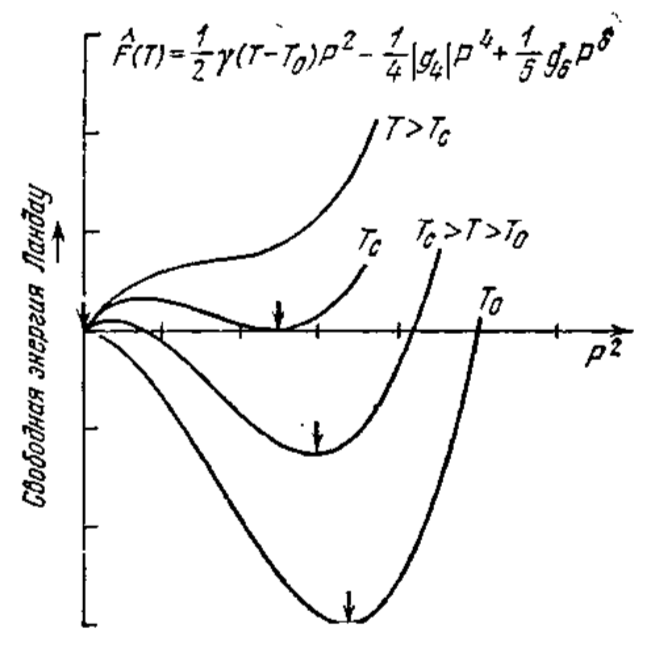
\includegraphics[scale = 0.7]{p7.png}
\caption{Свободная энергия как функция квадрата поляризации при различных типичных температурах (случай фазового перехода 1-го рода). При переходе T через $T_c$ положение абсолютного минимума изменяется скачком. }
\label{p7}
\end{center}
\end{figure}

На рис. \ref{p7} показан типичный ход изменения $P_s$ с температурой при фазовом переходе 1-го рода; видно, что картина совсем иная, чем в случай перехода 2-го рода (рис. \ref{p5}). 

\

Диэлектрическая проницаемость вычисляется из величины равновесной поляризации при данном значении внешнего электрического поля $\vec{E}$ согласно формуле (\ref{10}). При температурах выше точки Кюри в состоянии равновесия членами порядка $P^4$ и $P^6$ можно пренебречь; тогда:

\begin{equation}
E = \alpha'_{T_c} (T - T_c)P,
\label{26}
\end{equation}

или (для $T > T_c$):

\begin{equation}
\varepsilon = 1+ 4\pi \frac{P}{E} = 1 + \frac{4\pi}{\alpha'_{T_c} (T - T_c)}
\label{27}
\end{equation}

Закон Кюри-Вейсса (\ref{27}) имеет такой же аналитический вид (\ref{22}), однако проявляет особенности. Если ФП-2 происходит при $T = T_c$ и $\alpha = 0$, то для ФП-1  $\alpha \neq 0$, а имеет значение:

\begin{equation}
\alpha = \frac{3 \beta^2}{16 \gamma},
\label{27}
\end{equation}

где $\gamma > 0$. 

Отсюда следует, что $T'_c$ в случае с ФП-1 будет больше, чем $T_c$. Спонтанная поляризованность при $T = T'_c$ возникает скачком. 

Величина этого скачка $\Delta P^2_s = \frac{3 \beta}{4 \gamma}$. Скачком при $T'_c$ изменяется и величина $\varepsilon$, которая в точке ФП-1 имеет вполне определенное, не бесконечное, как при ФП-2, а максимальное значение, равное $\frac{16\gamma}{3\beta^2}$. На рис. \ref{p7} показаны температурные зависимости $P_s$ и $\varepsilon$ в сегнетоэлектриках с ФП-1. 

\begin{figure}[H]
\begin{center}
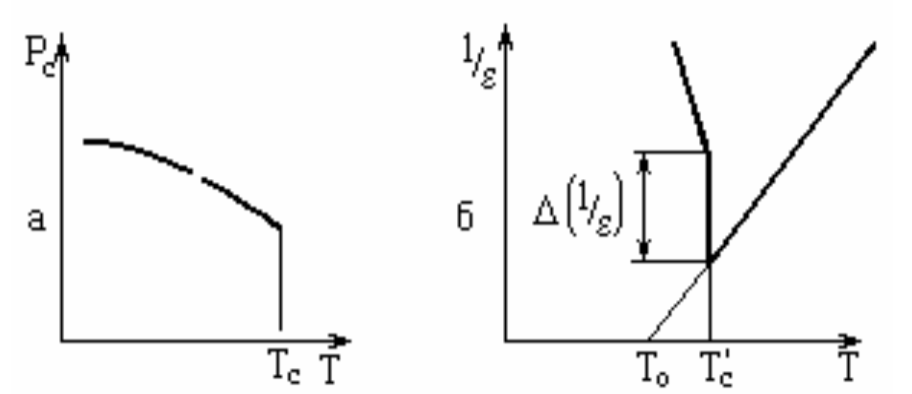
\includegraphics[scale = 0.7]{p8.png}
\caption{Температурная зависимость спонтанной поляризации (а) и обратной диэлектрической проницаемости (б) в сегнетоэлектриках с ФП-2. $T'_c$ - точка Кюри, $T_c$ - температура Кюри-Вейсса. }
\label{p7}
\end{center}
\end{figure}

\section{Фазовый переход в титанате бария}

Рассмотрим поведение сегнетоэлектриков на примере титаната бария, так как он имеет наиболее простую кристаллическую структуру. 

\begin{itemize}

\item

В неполярной фазе выше 120 $^{\circ} C$ это есть кубическая структура перовскита (рис. \ref{p2} слева).  Ввиду наличия центра симметрии титанат бария в неполярной фазе не обладает пьезоэлектрическими свойствами. 

\begin{figure}[H]
\begin{center}
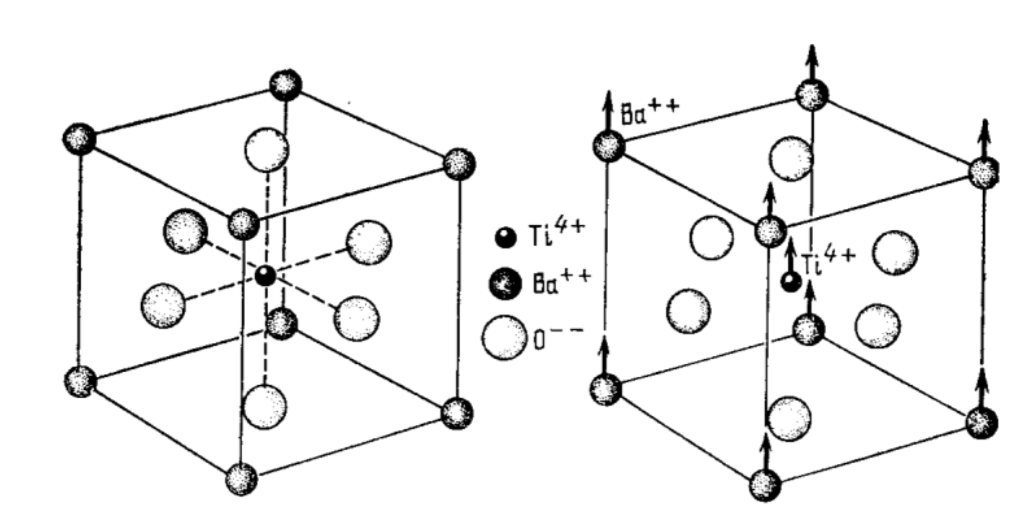
\includegraphics[scale = 0.7]{p2.png}

\caption{Перовскитная структура титаната бария слева; Деформированная структура справа}
\label{p2}
\end{center}
\end{figure}

\item

В полярной области температур между точкой Кюри (120 $^{\circ} C$) и температурой 5 $^{\circ} C$ имеют тетрагональную симметрию и становятся пьезоэлектриками. (рис. \ref{p2} справа)

Фазовый переход сводится к тому, что одно из ребер кубической ячейки удлиняется и становится полярной тетрагональной осью симметрии, обозначенной \textbf{c}, два других ребра одинаково укорачиваются, перезодя в тетрагональные оси - \textbf{a} (рис. \ref{p3})

\begin{figure}[h]
\begin{center}
\begin{minipage}[h]{0.4\linewidth}
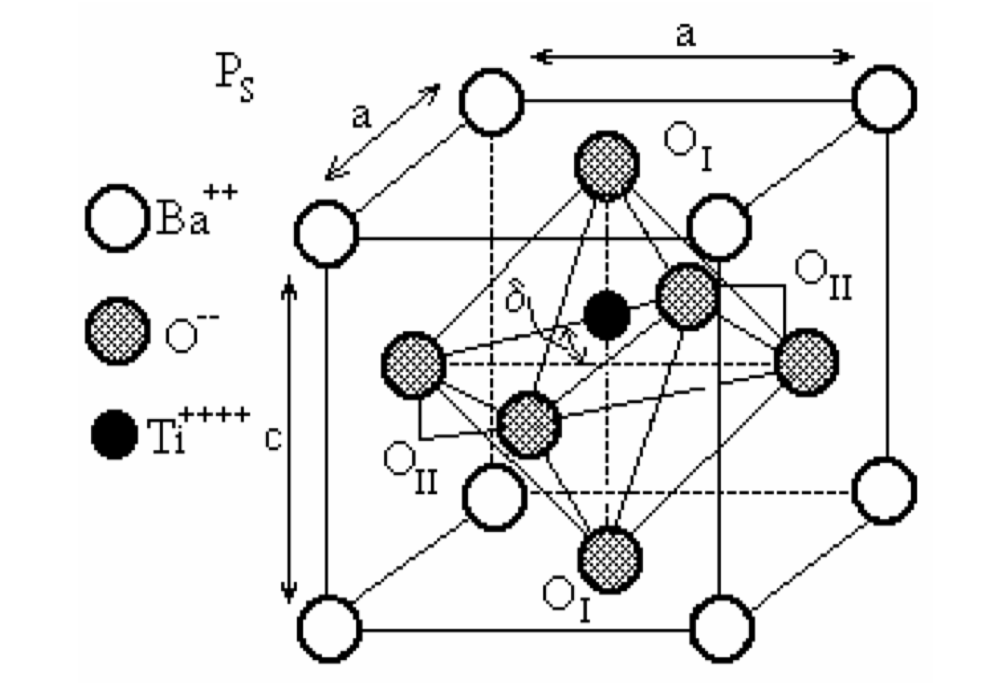
\includegraphics[width=1\linewidth]{p3.png}
\caption{Тетрагональная струтура} %% подпись к рисунку
\label{p3} %% метка рисунка для ссылки на него
\end{minipage}
\hfill 
\begin{minipage}[h]{0.4\linewidth}
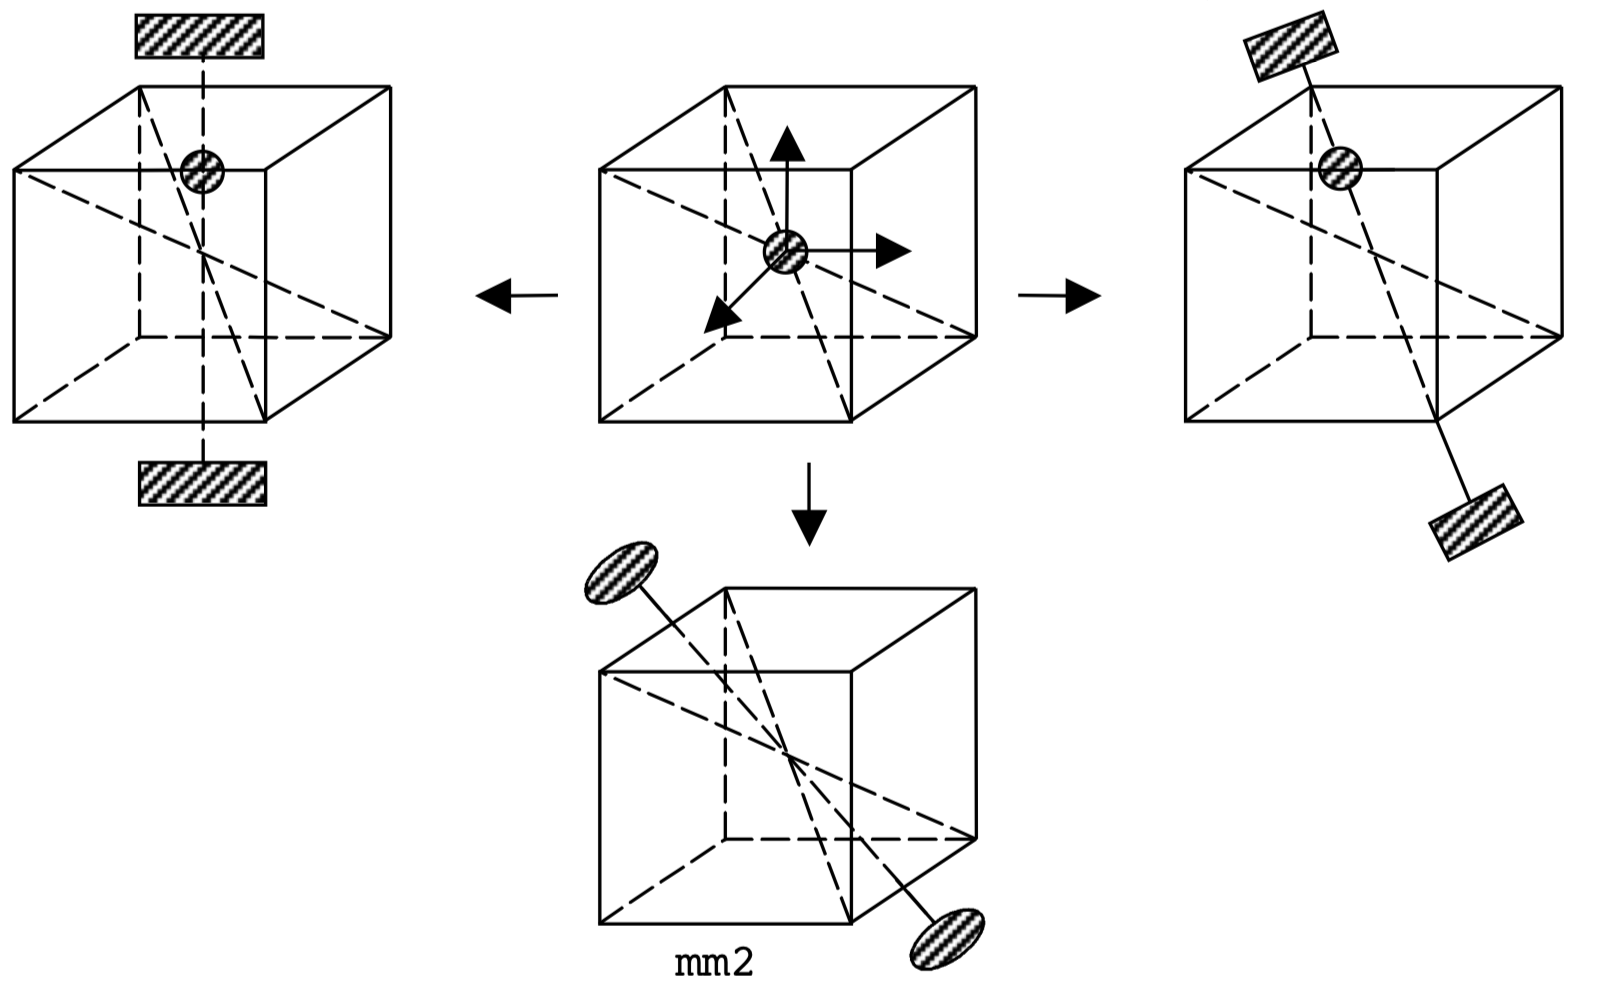
\includegraphics[width=1\linewidth]{p9.png}
\caption{Тетрагонгальная (слева); ромбоэдрическая (справа); орторомбическая (снизу)}
\label{p9}
\end{minipage}
\end{center}
\end{figure}


Поскольку все три ребра эквивалентны, каждое из низ может перейти в полярную ось. Существует 6 возможных направлений. 
\item 

Ниже 5$^{\circ} C$ титанат бария испытвает второе фазовое превращение. Получается новая сегнетоэлектрическая фаза, устойчивая между 5 и -90 $^{\circ} C$ и обладающая орторомбической симметрией. 

Конфигурация может быть получена из исходной кубической ячейки, если ее растянуть вдоль диагонали одной из граней куба и сжать вдоль другой диагонали той же грани. Растянутая диагональ служит полярной осью кристалла. Существует 12 направлений. 

\item

При -90 $^{\circ} C$ происходит третий фазовый переход. Кристалл становиться ромбоэдрическим с полярной осью вдоль вдоль одной из пространственных диагоналей куба. Так как исходная кубическая ячейка содержит четыре эквивалентных пространственных диагонали, то в ромбоэдрической фазе существует восемь направлений спонтанной поляризации. 

\end{itemize}

В кристаллах титаната бария в электрическом поле границы доменов смещаются в результате последовательного зарождения доменов вдоль плоскости исходной стенки за счет тепловых флуктуация. Скорость зародышеобразования является основным фактором, определяющим движение стенки, - ситуация совершенно не похожая на ту, что имеем для ферромагнитных доменов. 

\section{Сегнетоэлектрическая память}

Итак, сделаем обобщение всех "замечательных" свойств сегнетоэлектрика:
\begin{itemize}

\item

Имеют место фазовые переходы \RNumb{1} и \RNumb{2} рода как следствие переход из параэлектрического состояния в полярное. 

\item

Сегнетоэлектрик обладает нелинейной связью между приложенным электрическим полем и хранимым зарядом в полярной фазе.
 
\item

В частности, сегнетоэлектрическая характеристика имеет вид петли гистерезиса, который очень схож с в общих чертах с петлёй гистерезиса ферромагнитных материалов. 

\item

Диэлектрическая константа сегнетоэлектрика, как правило, значительно выше, чем у линейного диэлектрика. 

\item

После удаления внешнего поля диполи сохраняют своё состояние поляризации. 

\end{itemize}

В частности гистерезис позволяет иметь два устойчивых состояния, которые можно интерпретировать как <<0>> и <<1>>. 

Обычно двоичные «0» и «1» хранятся в виде одной из двух возможных электрических поляризаций в каждой ячейке хранения данных. Например, под «1» понимается отрицательный остаток поляризации $-P_r$, а под «0» — положительный остаток поляризации $+P_r$.

\

Рассмотрим самую простую схему FeRAM с одним конденсатором и транзистором (рис. \ref{p10}). Отметим, что направление поляризации в конденсаторе определяется направлением приложенного напряжения (рис. \ref{p14})

\begin{figure}[H]
\begin{center}
\begin{minipage}[h]{0.35\linewidth}
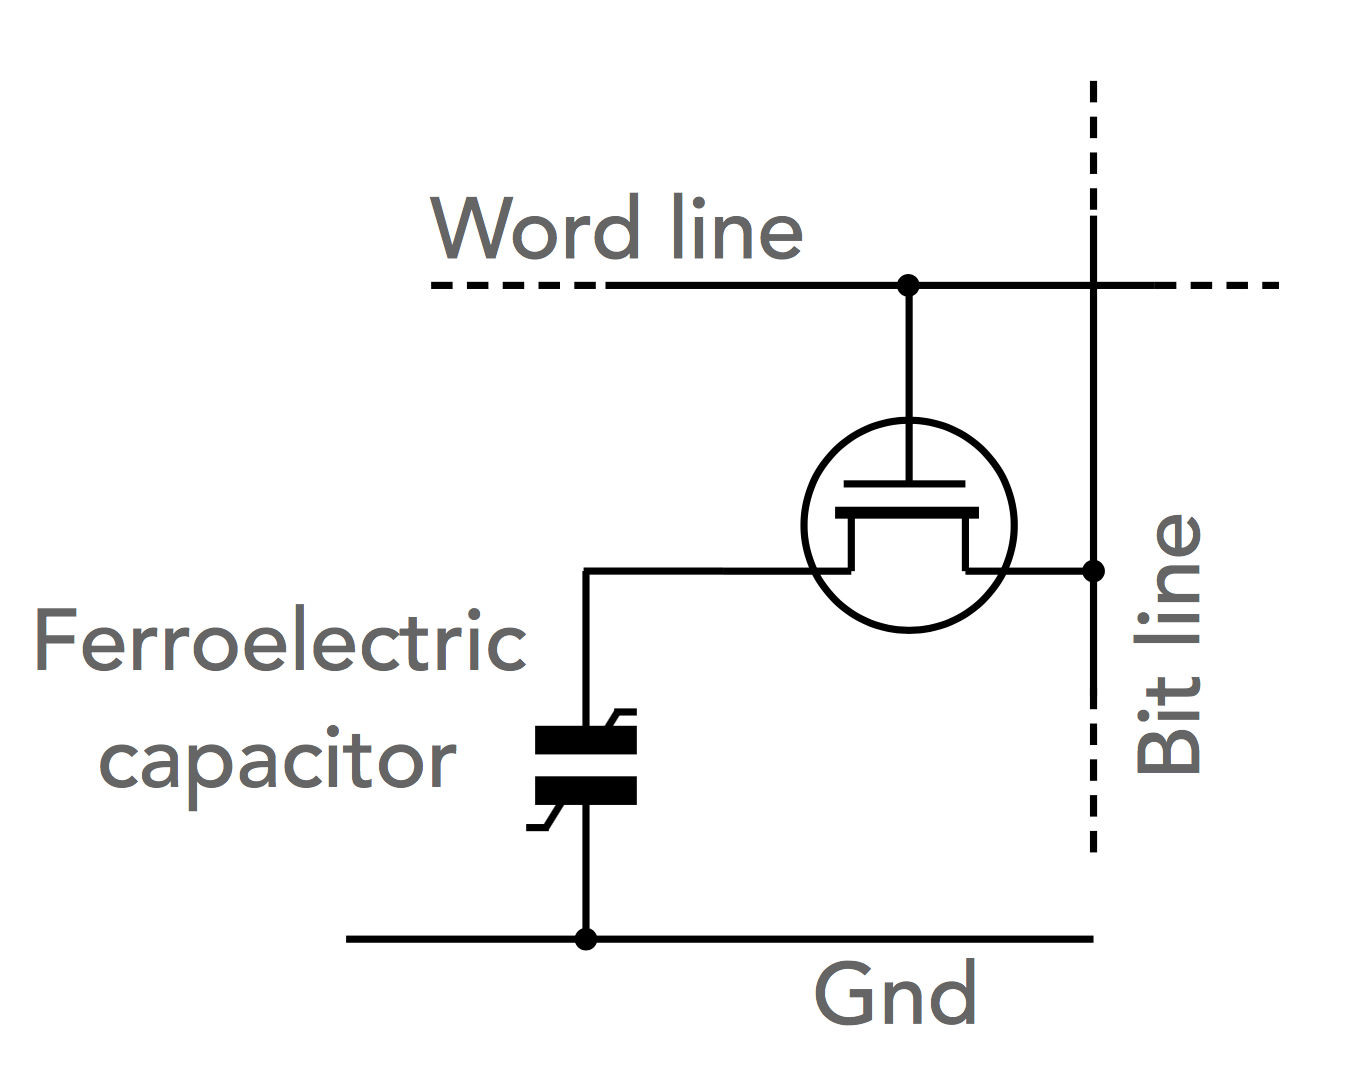
\includegraphics[width=1\linewidth]{p10.png}
\caption{Схема  ячейки 1Т-1С} %% подпись к рисунку
\label{p10} %% метка рисунка для ссылки на него
\end{minipage}
\hfill 
\begin{minipage}[h]{0.4\linewidth}
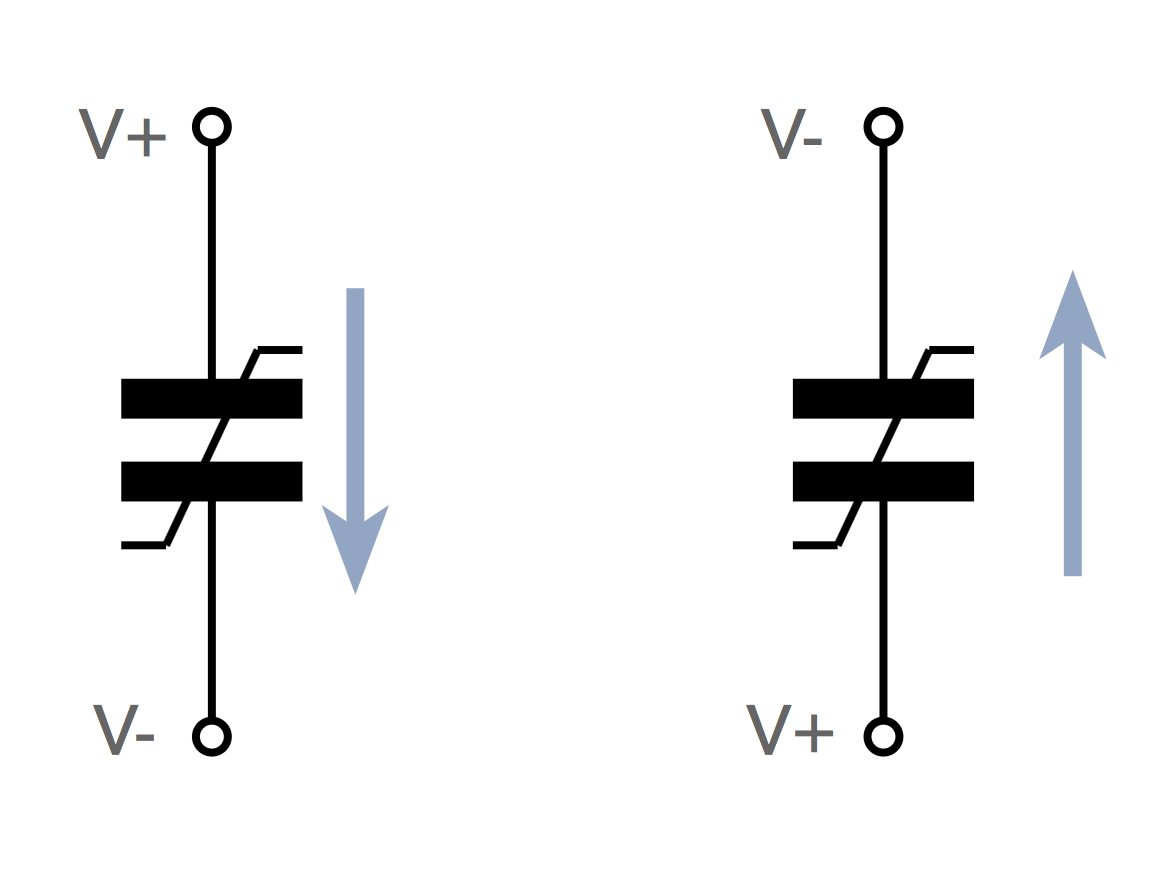
\includegraphics[width=1\linewidth]{p14.png}
\caption{Направление поляризации в зависимости от направления напряжения}
\label{p14}
\end{minipage}
\end{center}
\end{figure}

Функционально FeRAM похожа на DRAM. Запись происходит путём проникновения поля через сегнетоэлектрический слой при заряжании электродов, принуждая атомы внутри принимать ориентацию вверх или вниз (в зависимости от полярности заряда), за счёт чего запоминается <<1>> или <<0>>. Однако принцип чтения отличается от реализации в DRAM. 

Сначала все три линии становятся неактивными <<0>> (рис. \ref{p11}). Считывание начинается с того, что на 2 линии подается напряжение (рис. \ref{p12}), далее возможны 2 случая:

\begin{itemize}

\item

Если ячейка уже содержит <<0>> (то есть направление поляризации согласовано с направлением напряжения), то на линиях вывода ничего не произойдет.

\item

Если ячейка содержала <<1>> (направление поляризации не согласовано) (рис. \ref{p13}), то переориентация атомов в прослойке приведет к короткому импульсу на выходе, так как они вытолкнут электроны из металла. Наличие этого импульса будет означать, что ячейка хранит <<1>>. Так как процесс перезаписывает содержимое ячейки, то чтение из FeRAM — деструктивный процесс, и требует регенерации данных в ячейке в случае их изменения в ходе считывания.

\end{itemize}

\begin{figure}[H]
\begin{center}
\begin{minipage}[h]{0.32\linewidth}
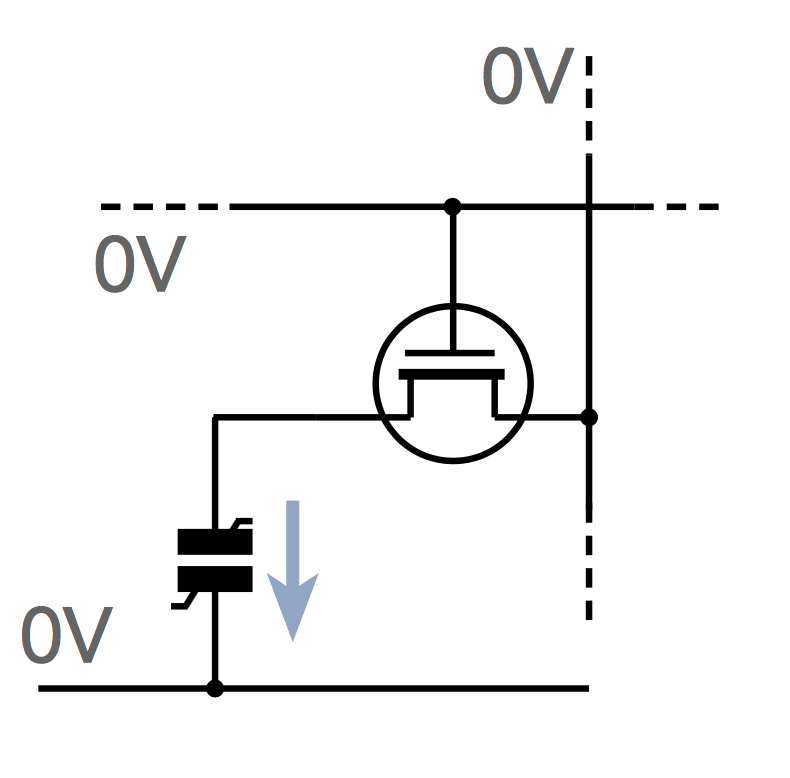
\includegraphics[width=0.9\linewidth]{p11.png}
\caption{} 
\label{p11} 
\end{minipage}
\hfill 
\begin{minipage}[h]{0.32\linewidth}
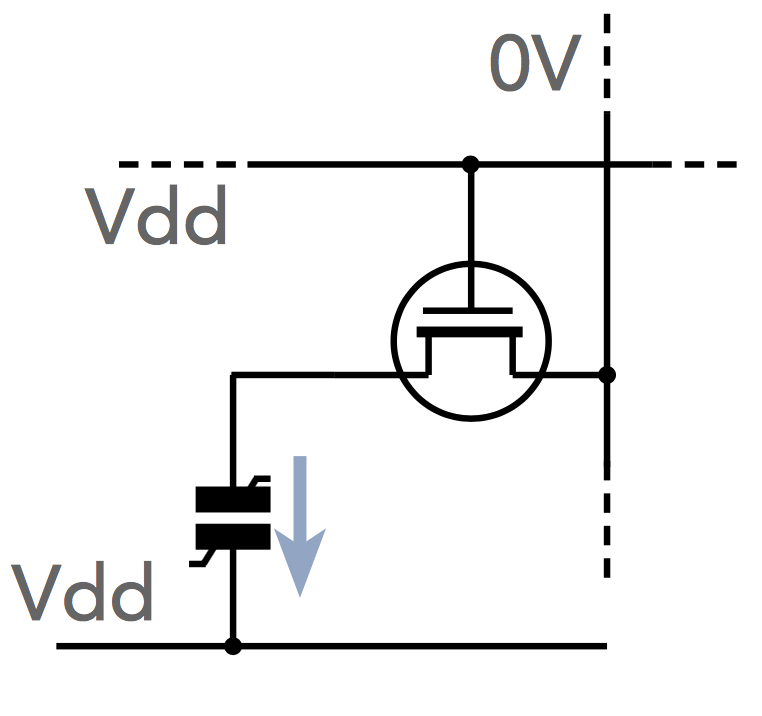
\includegraphics[width=0.9\linewidth]{p12.png}
\caption{}
\label{p12}
\end{minipage}
\hfill 
\begin{minipage}[h]{0.32\linewidth}
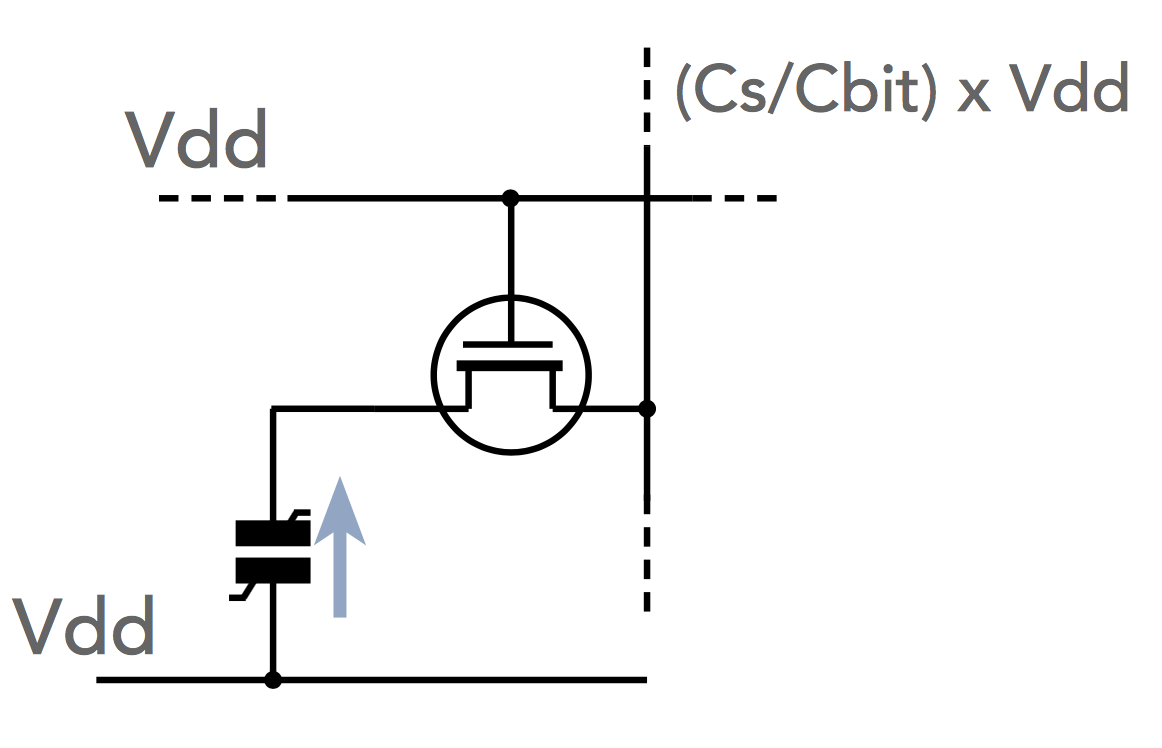
\includegraphics[width=1.5\linewidth]{p13.png}
\caption{}
\label{p13}
\end{minipage}
\end{center}
\end{figure}


\section{Литература и источники}

\begin{enumerate}

\item

Сивухин Д.В. Общий курс физики. Т. \RNumb{3}. Электричество. - М.: ФИЗМАТЛИТ, 2016. - § 39. - C. 162 - 173. 

\item

К.А. Воротилов, А.С. Сигов Физика твердого тела, 2012, том 54, вып. 5

\item

Методическое пособие "Фазовый переход в сегнетоэлектриках". Неизвестный автор. 

\item

Васильева Д.С. Диссертация "Сегнетоэлектрические и пьезоэлектрические свойства и фазовые превращения в кристаллах глицина". Екатеринбург - 2018

\item

Ляпин А. Г. Лабораторная работа № 24 "Фазовый переход в сегнетоэлектрике"  МФТИ. 

\item

Желудев И.С. Основы сегнетоэлектричества. М.: Атомиздат, 1973. 471с.

\item

$https://www.electronics-notes.com/articles/electronic_components/semiconductor-ic-memory/fram-ferroelectric-ram-operation-technology.php$

\item

$https://ru.wikipedia.org/wiki/FRAM$

\item

$http://gete.ru/post_1173901482.html$

\end{enumerate}

\end{document}